% Graphic for TeX using PGF
% Title: /home/satenske/cours/AP/obj3/uml5.dia
% Creator: Dia v0.97.1
% CreationDate: Thu Sep 22 10:08:42 2011
% For: satenske
% \usepackage{tikz}
% The following commands are not supported in PSTricks at present
% We define them conditionally, so when they are implemented,
% this pgf file will use them.
\ifx\du\undefined
  \newlength{\du}
\fi
\setlength{\du}{15\unitlength}
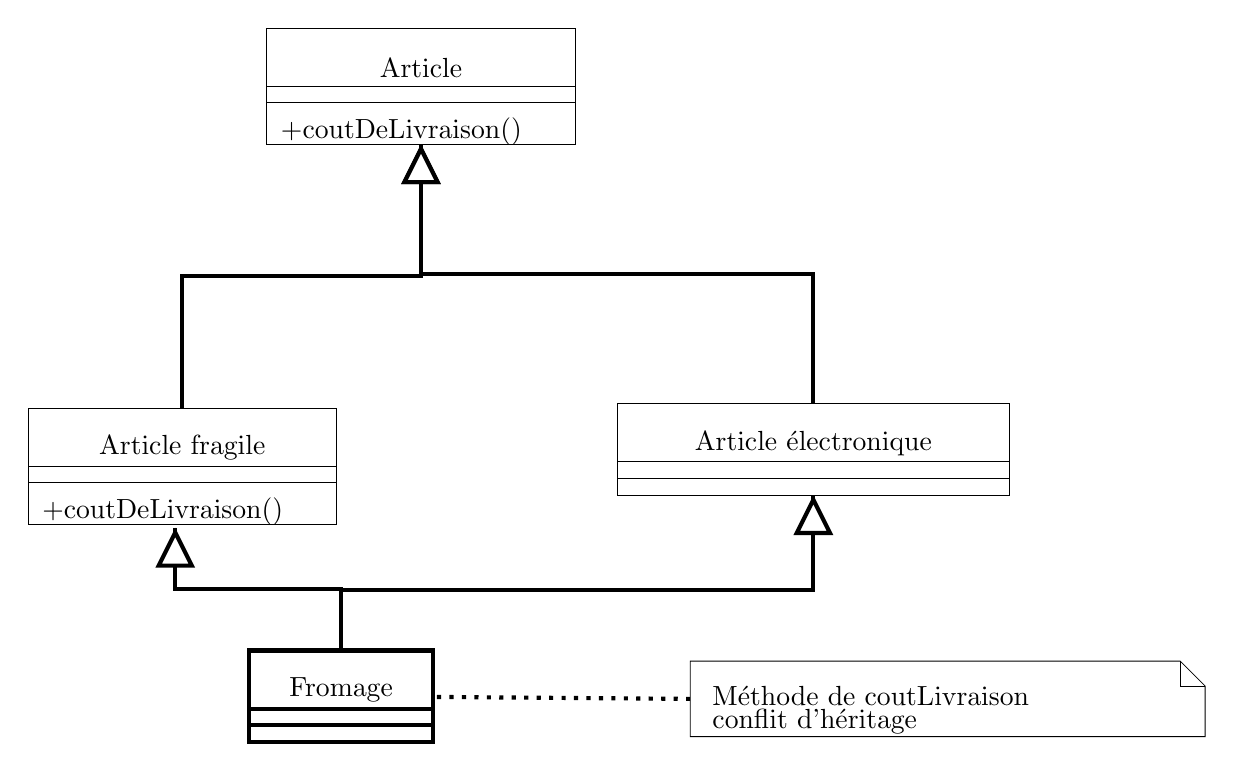
\begin{tikzpicture}
\pgftransformxscale{1.000000}
\pgftransformyscale{-1.000000}
\definecolor{dialinecolor}{rgb}{0.000000, 0.000000, 0.000000}
\pgfsetstrokecolor{dialinecolor}
\definecolor{dialinecolor}{rgb}{1.000000, 1.000000, 1.000000}
\pgfsetfillcolor{dialinecolor}
\pgfsetlinewidth{0.020000\du}
\pgfsetdash{}{0pt}
\definecolor{dialinecolor}{rgb}{1.000000, 1.000000, 1.000000}
\pgfsetfillcolor{dialinecolor}
\fill (9.600000\du,1.050000\du)--(9.600000\du,2.450000\du)--(17.030000\du,2.450000\du)--(17.030000\du,1.050000\du)--cycle;
\definecolor{dialinecolor}{rgb}{0.000000, 0.000000, 0.000000}
\pgfsetstrokecolor{dialinecolor}
\draw (9.600000\du,1.050000\du)--(9.600000\du,2.450000\du)--(17.030000\du,2.450000\du)--(17.030000\du,1.050000\du)--cycle;
% setfont left to latex
\definecolor{dialinecolor}{rgb}{0.000000, 0.000000, 0.000000}
\pgfsetstrokecolor{dialinecolor}
\node at (13.315000\du,2.000000\du){Article};
\definecolor{dialinecolor}{rgb}{1.000000, 1.000000, 1.000000}
\pgfsetfillcolor{dialinecolor}
\fill (9.600000\du,2.450000\du)--(9.600000\du,2.850000\du)--(17.030000\du,2.850000\du)--(17.030000\du,2.450000\du)--cycle;
\definecolor{dialinecolor}{rgb}{0.000000, 0.000000, 0.000000}
\pgfsetstrokecolor{dialinecolor}
\draw (9.600000\du,2.450000\du)--(9.600000\du,2.850000\du)--(17.030000\du,2.850000\du)--(17.030000\du,2.450000\du)--cycle;
\definecolor{dialinecolor}{rgb}{1.000000, 1.000000, 1.000000}
\pgfsetfillcolor{dialinecolor}
\fill (9.600000\du,2.850000\du)--(9.600000\du,3.850000\du)--(17.030000\du,3.850000\du)--(17.030000\du,2.850000\du)--cycle;
\definecolor{dialinecolor}{rgb}{0.000000, 0.000000, 0.000000}
\pgfsetstrokecolor{dialinecolor}
\draw (9.600000\du,2.850000\du)--(9.600000\du,3.850000\du)--(17.030000\du,3.850000\du)--(17.030000\du,2.850000\du)--cycle;
% setfont left to latex
\definecolor{dialinecolor}{rgb}{0.000000, 0.000000, 0.000000}
\pgfsetstrokecolor{dialinecolor}
\node[anchor=west] at (9.710000\du,3.550000\du){+coutDeLivraison()};
\pgfsetlinewidth{0.020000\du}
\pgfsetdash{}{0pt}
\definecolor{dialinecolor}{rgb}{1.000000, 1.000000, 1.000000}
\pgfsetfillcolor{dialinecolor}
\fill (18.050000\du,10.100000\du)--(18.050000\du,11.500000\du)--(27.485000\du,11.500000\du)--(27.485000\du,10.100000\du)--cycle;
\definecolor{dialinecolor}{rgb}{0.000000, 0.000000, 0.000000}
\pgfsetstrokecolor{dialinecolor}
\draw (18.050000\du,10.100000\du)--(18.050000\du,11.500000\du)--(27.485000\du,11.500000\du)--(27.485000\du,10.100000\du)--cycle;
% setfont left to latex
\definecolor{dialinecolor}{rgb}{0.000000, 0.000000, 0.000000}
\pgfsetstrokecolor{dialinecolor}
\node at (22.767500\du,11.050000\du){Article électronique};
\definecolor{dialinecolor}{rgb}{1.000000, 1.000000, 1.000000}
\pgfsetfillcolor{dialinecolor}
\fill (18.050000\du,11.500000\du)--(18.050000\du,11.900000\du)--(27.485000\du,11.900000\du)--(27.485000\du,11.500000\du)--cycle;
\definecolor{dialinecolor}{rgb}{0.000000, 0.000000, 0.000000}
\pgfsetstrokecolor{dialinecolor}
\draw (18.050000\du,11.500000\du)--(18.050000\du,11.900000\du)--(27.485000\du,11.900000\du)--(27.485000\du,11.500000\du)--cycle;
\definecolor{dialinecolor}{rgb}{1.000000, 1.000000, 1.000000}
\pgfsetfillcolor{dialinecolor}
\fill (18.050000\du,11.900000\du)--(18.050000\du,12.300000\du)--(27.485000\du,12.300000\du)--(27.485000\du,11.900000\du)--cycle;
\definecolor{dialinecolor}{rgb}{0.000000, 0.000000, 0.000000}
\pgfsetstrokecolor{dialinecolor}
\draw (18.050000\du,11.900000\du)--(18.050000\du,12.300000\du)--(27.485000\du,12.300000\du)--(27.485000\du,11.900000\du)--cycle;
\pgfsetlinewidth{0.020000\du}
\pgfsetdash{}{0pt}
\definecolor{dialinecolor}{rgb}{1.000000, 1.000000, 1.000000}
\pgfsetfillcolor{dialinecolor}
\fill (3.850000\du,10.200000\du)--(3.850000\du,11.600000\du)--(11.280000\du,11.600000\du)--(11.280000\du,10.200000\du)--cycle;
\definecolor{dialinecolor}{rgb}{0.000000, 0.000000, 0.000000}
\pgfsetstrokecolor{dialinecolor}
\draw (3.850000\du,10.200000\du)--(3.850000\du,11.600000\du)--(11.280000\du,11.600000\du)--(11.280000\du,10.200000\du)--cycle;
% setfont left to latex
\definecolor{dialinecolor}{rgb}{0.000000, 0.000000, 0.000000}
\pgfsetstrokecolor{dialinecolor}
\node at (7.565000\du,11.150000\du){Article fragile};
\definecolor{dialinecolor}{rgb}{1.000000, 1.000000, 1.000000}
\pgfsetfillcolor{dialinecolor}
\fill (3.850000\du,11.600000\du)--(3.850000\du,12.000000\du)--(11.280000\du,12.000000\du)--(11.280000\du,11.600000\du)--cycle;
\definecolor{dialinecolor}{rgb}{0.000000, 0.000000, 0.000000}
\pgfsetstrokecolor{dialinecolor}
\draw (3.850000\du,11.600000\du)--(3.850000\du,12.000000\du)--(11.280000\du,12.000000\du)--(11.280000\du,11.600000\du)--cycle;
\definecolor{dialinecolor}{rgb}{1.000000, 1.000000, 1.000000}
\pgfsetfillcolor{dialinecolor}
\fill (3.850000\du,12.000000\du)--(3.850000\du,13.000000\du)--(11.280000\du,13.000000\du)--(11.280000\du,12.000000\du)--cycle;
\definecolor{dialinecolor}{rgb}{0.000000, 0.000000, 0.000000}
\pgfsetstrokecolor{dialinecolor}
\draw (3.850000\du,12.000000\du)--(3.850000\du,13.000000\du)--(11.280000\du,13.000000\du)--(11.280000\du,12.000000\du)--cycle;
% setfont left to latex
\definecolor{dialinecolor}{rgb}{0.000000, 0.000000, 0.000000}
\pgfsetstrokecolor{dialinecolor}
\node[anchor=west] at (3.960000\du,12.700000\du){+coutDeLivraison()};
\pgfsetlinewidth{0.020000\du}
\pgfsetdash{}{0pt}
\definecolor{dialinecolor}{rgb}{1.000000, 1.000000, 1.000000}
\pgfsetfillcolor{dialinecolor}
\fill (19.800000\du,16.300000\du)--(31.605000\du,16.300000\du)--(32.205000\du,16.900000\du)--(32.205000\du,18.118633\du)--(19.800000\du,18.118633\du)--cycle;
\definecolor{dialinecolor}{rgb}{0.000000, 0.000000, 0.000000}
\pgfsetstrokecolor{dialinecolor}
\draw (19.800000\du,16.300000\du)--(31.605000\du,16.300000\du)--(32.205000\du,16.900000\du)--(32.205000\du,18.118633\du)--(19.800000\du,18.118633\du)--cycle;
\pgfsetlinewidth{0.010000\du}
\definecolor{dialinecolor}{rgb}{0.000000, 0.000000, 0.000000}
\pgfsetstrokecolor{dialinecolor}
\draw (31.605000\du,16.300000\du)--(31.605000\du,16.900000\du)--(32.205000\du,16.900000\du);
% setfont left to latex
\definecolor{dialinecolor}{rgb}{0.000000, 0.000000, 0.000000}
\pgfsetstrokecolor{dialinecolor}
\node[anchor=west] at (20.110000\du,17.137500\du){Méthode de coutLivraison                                                      };
% setfont left to latex
\definecolor{dialinecolor}{rgb}{0.000000, 0.000000, 0.000000}
\pgfsetstrokecolor{dialinecolor}
\node[anchor=west] at (20.110000\du,17.443711\du){};
% setfont left to latex
\definecolor{dialinecolor}{rgb}{0.000000, 0.000000, 0.000000}
\pgfsetstrokecolor{dialinecolor}
\node[anchor=west] at (20.110000\du,17.749922\du){conflit d'héritage                                };
\pgfsetlinewidth{0.100000\du}
\pgfsetdash{}{0pt}
\definecolor{dialinecolor}{rgb}{1.000000, 1.000000, 1.000000}
\pgfsetfillcolor{dialinecolor}
\fill (9.175000\du,16.045000\du)--(9.175000\du,17.445000\du)--(13.605000\du,17.445000\du)--(13.605000\du,16.045000\du)--cycle;
\definecolor{dialinecolor}{rgb}{0.000000, 0.000000, 0.000000}
\pgfsetstrokecolor{dialinecolor}
\draw (9.175000\du,16.045000\du)--(9.175000\du,17.445000\du)--(13.605000\du,17.445000\du)--(13.605000\du,16.045000\du)--cycle;
% setfont left to latex
\definecolor{dialinecolor}{rgb}{0.000000, 0.000000, 0.000000}
\pgfsetstrokecolor{dialinecolor}
\node at (11.390000\du,16.995000\du){Fromage};
\definecolor{dialinecolor}{rgb}{1.000000, 1.000000, 1.000000}
\pgfsetfillcolor{dialinecolor}
\fill (9.175000\du,17.445000\du)--(9.175000\du,17.845000\du)--(13.605000\du,17.845000\du)--(13.605000\du,17.445000\du)--cycle;
\definecolor{dialinecolor}{rgb}{0.000000, 0.000000, 0.000000}
\pgfsetstrokecolor{dialinecolor}
\draw (9.175000\du,17.445000\du)--(9.175000\du,17.845000\du)--(13.605000\du,17.845000\du)--(13.605000\du,17.445000\du)--cycle;
\definecolor{dialinecolor}{rgb}{1.000000, 1.000000, 1.000000}
\pgfsetfillcolor{dialinecolor}
\fill (9.175000\du,17.845000\du)--(9.175000\du,18.245000\du)--(13.605000\du,18.245000\du)--(13.605000\du,17.845000\du)--cycle;
\definecolor{dialinecolor}{rgb}{0.000000, 0.000000, 0.000000}
\pgfsetstrokecolor{dialinecolor}
\draw (9.175000\du,17.845000\du)--(9.175000\du,18.245000\du)--(13.605000\du,18.245000\du)--(13.605000\du,17.845000\du)--cycle;
\pgfsetlinewidth{0.100000\du}
\pgfsetdash{}{0pt}
\pgfsetmiterjoin
\pgfsetbuttcap
{
\definecolor{dialinecolor}{rgb}{0.000000, 0.000000, 0.000000}
\pgfsetfillcolor{dialinecolor}
% was here!!!
\definecolor{dialinecolor}{rgb}{0.000000, 0.000000, 0.000000}
\pgfsetstrokecolor{dialinecolor}
\draw (13.315000\du,3.850000\du)--(13.315000\du,7.025000\du)--(7.565000\du,7.025000\du)--(7.565000\du,10.200000\du);
}
\definecolor{dialinecolor}{rgb}{0.000000, 0.000000, 0.000000}
\pgfsetstrokecolor{dialinecolor}
\draw (13.315000\du,4.761803\du)--(13.315000\du,7.025000\du)--(7.565000\du,7.025000\du)--(7.565000\du,10.200000\du);
\pgfsetmiterjoin
\definecolor{dialinecolor}{rgb}{1.000000, 1.000000, 1.000000}
\pgfsetfillcolor{dialinecolor}
\fill (13.715000\du,4.761803\du)--(13.315000\du,3.961803\du)--(12.915000\du,4.761803\du)--cycle;
\pgfsetlinewidth{0.100000\du}
\pgfsetdash{}{0pt}
\pgfsetmiterjoin
\definecolor{dialinecolor}{rgb}{0.000000, 0.000000, 0.000000}
\pgfsetstrokecolor{dialinecolor}
\draw (13.715000\du,4.761803\du)--(13.315000\du,3.961803\du)--(12.915000\du,4.761803\du)--cycle;
% setfont left to latex
\pgfsetlinewidth{0.100000\du}
\pgfsetdash{}{0pt}
\pgfsetmiterjoin
\pgfsetbuttcap
{
\definecolor{dialinecolor}{rgb}{0.000000, 0.000000, 0.000000}
\pgfsetfillcolor{dialinecolor}
% was here!!!
\definecolor{dialinecolor}{rgb}{0.000000, 0.000000, 0.000000}
\pgfsetstrokecolor{dialinecolor}
\draw (13.315000\du,3.850000\du)--(13.315000\du,6.975000\du)--(22.767500\du,6.975000\du)--(22.767500\du,10.100000\du);
}
\definecolor{dialinecolor}{rgb}{0.000000, 0.000000, 0.000000}
\pgfsetstrokecolor{dialinecolor}
\draw (13.315000\du,4.761803\du)--(13.315000\du,6.975000\du)--(22.767500\du,6.975000\du)--(22.767500\du,10.100000\du);
\pgfsetmiterjoin
\definecolor{dialinecolor}{rgb}{1.000000, 1.000000, 1.000000}
\pgfsetfillcolor{dialinecolor}
\fill (13.715000\du,4.761803\du)--(13.315000\du,3.961803\du)--(12.915000\du,4.761803\du)--cycle;
\pgfsetlinewidth{0.100000\du}
\pgfsetdash{}{0pt}
\pgfsetmiterjoin
\definecolor{dialinecolor}{rgb}{0.000000, 0.000000, 0.000000}
\pgfsetstrokecolor{dialinecolor}
\draw (13.715000\du,4.761803\du)--(13.315000\du,3.961803\du)--(12.915000\du,4.761803\du)--cycle;
% setfont left to latex
\pgfsetlinewidth{0.100000\du}
\pgfsetdash{}{0pt}
\pgfsetmiterjoin
\pgfsetbuttcap
{
\definecolor{dialinecolor}{rgb}{0.000000, 0.000000, 0.000000}
\pgfsetfillcolor{dialinecolor}
% was here!!!
\definecolor{dialinecolor}{rgb}{0.000000, 0.000000, 0.000000}
\pgfsetstrokecolor{dialinecolor}
\draw (7.395100\du,13.087500\du)--(7.395100\du,14.566250\du)--(11.390000\du,14.566250\du)--(11.390000\du,16.045000\du);
}
\definecolor{dialinecolor}{rgb}{0.000000, 0.000000, 0.000000}
\pgfsetstrokecolor{dialinecolor}
\draw (7.395100\du,13.999303\du)--(7.395100\du,14.566250\du)--(11.390000\du,14.566250\du)--(11.390000\du,16.045000\du);
\pgfsetmiterjoin
\definecolor{dialinecolor}{rgb}{1.000000, 1.000000, 1.000000}
\pgfsetfillcolor{dialinecolor}
\fill (7.795100\du,13.999303\du)--(7.395100\du,13.199303\du)--(6.995100\du,13.999303\du)--cycle;
\pgfsetlinewidth{0.100000\du}
\pgfsetdash{}{0pt}
\pgfsetmiterjoin
\definecolor{dialinecolor}{rgb}{0.000000, 0.000000, 0.000000}
\pgfsetstrokecolor{dialinecolor}
\draw (7.795100\du,13.999303\du)--(7.395100\du,13.199303\du)--(6.995100\du,13.999303\du)--cycle;
% setfont left to latex
\pgfsetlinewidth{0.100000\du}
\pgfsetdash{}{0pt}
\pgfsetmiterjoin
\pgfsetbuttcap
{
\definecolor{dialinecolor}{rgb}{0.000000, 0.000000, 0.000000}
\pgfsetfillcolor{dialinecolor}
% was here!!!
\definecolor{dialinecolor}{rgb}{0.000000, 0.000000, 0.000000}
\pgfsetstrokecolor{dialinecolor}
\draw (22.767500\du,12.300000\du)--(22.767500\du,14.587500\du)--(11.390000\du,14.587500\du)--(11.390000\du,16.045000\du);
}
\definecolor{dialinecolor}{rgb}{0.000000, 0.000000, 0.000000}
\pgfsetstrokecolor{dialinecolor}
\draw (22.767500\du,13.211803\du)--(22.767500\du,14.587500\du)--(11.390000\du,14.587500\du)--(11.390000\du,16.045000\du);
\pgfsetmiterjoin
\definecolor{dialinecolor}{rgb}{1.000000, 1.000000, 1.000000}
\pgfsetfillcolor{dialinecolor}
\fill (23.167500\du,13.211803\du)--(22.767500\du,12.411803\du)--(22.367500\du,13.211803\du)--cycle;
\pgfsetlinewidth{0.100000\du}
\pgfsetdash{}{0pt}
\pgfsetmiterjoin
\definecolor{dialinecolor}{rgb}{0.000000, 0.000000, 0.000000}
\pgfsetstrokecolor{dialinecolor}
\draw (23.167500\du,13.211803\du)--(22.767500\du,12.411803\du)--(22.367500\du,13.211803\du)--cycle;
% setfont left to latex
\pgfsetlinewidth{0.100000\du}
\pgfsetdash{{\pgflinewidth}{0.200000\du}}{0cm}
\pgfsetdash{{\pgflinewidth}{0.200000\du}}{0cm}
\pgfsetbuttcap
{
\definecolor{dialinecolor}{rgb}{0.000000, 0.000000, 0.000000}
\pgfsetfillcolor{dialinecolor}
% was here!!!
\definecolor{dialinecolor}{rgb}{0.000000, 0.000000, 0.000000}
\pgfsetstrokecolor{dialinecolor}
\draw (19.800000\du,17.209317\du)--(13.611587\du,17.161990\du);
}
\end{tikzpicture}
